\section{Validação da Hipótese $H_1$: Paradigma Arquitetural}

Com o dataset V10 consolidado, avaliou-se a Hipótese $H_1$, que propõe a superioridade de arquiteturas de nova geração. A Figura \ref{fig:h1_paradigm} confronta o desempenho das CNNs e dos Transformers.

\begin{figure}[h!]
  \centering
  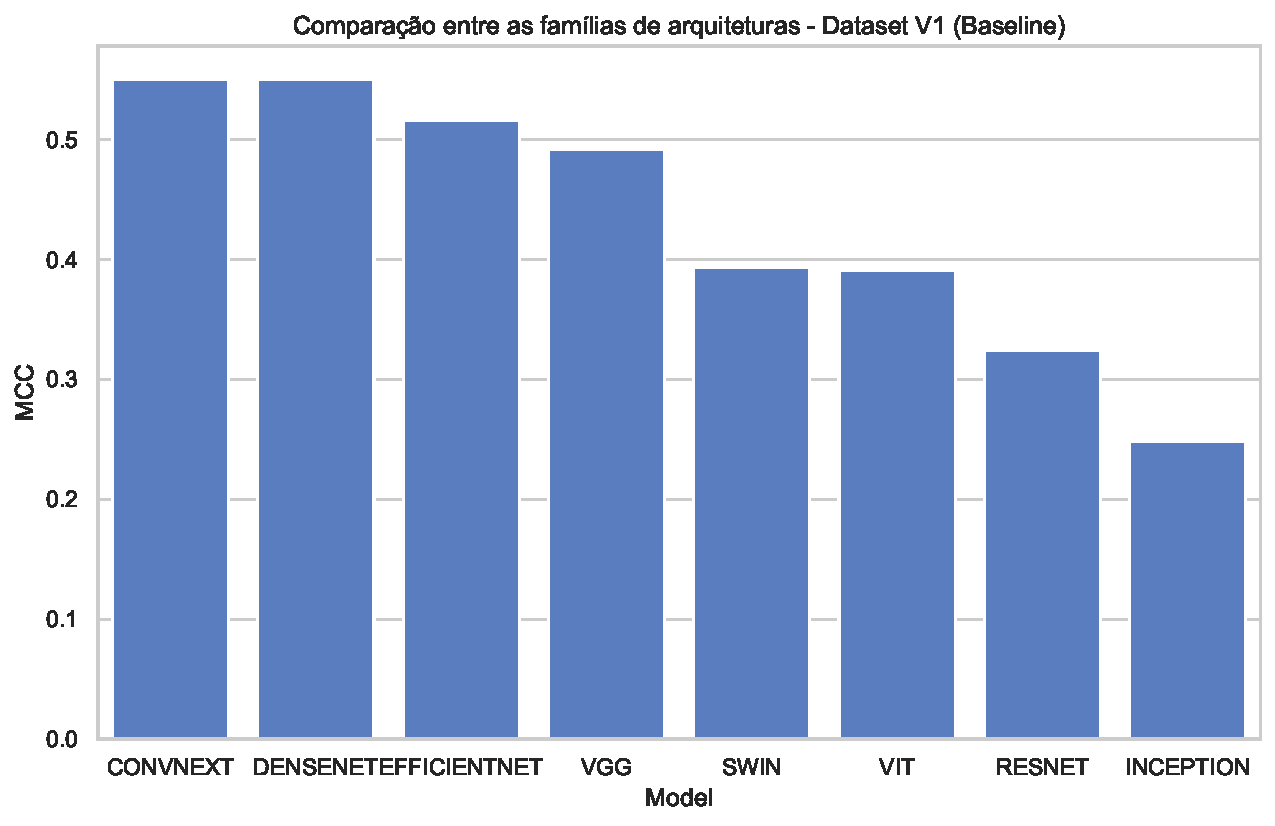
\includegraphics[width=0.8\textwidth]{images/h1_paradigm_comparison.pdf}
  \caption{Comparação de Paradigmas ($H_1$): CNNs vs. Transformers. Observa-se a liderança das CNNs densas e modernas.}
  \label{fig:h1_paradigm}
\end{figure}

Os resultados refutam a ideia de que Transformers puros (ViT) seriam superiores para este domínio. A média de MCC das CNNs foi significativamente superior à dos Transformers. Este comportamento sugere que para o reconhecimento de texturas da fibra de algodão, o viés indutivo de localidade das convoluções é mais eficaz que o mecanismo de atenção global, confirmando parcialmente $H_1$ apenas para a subfamília de CNNs modernas como a ConvNext.
